\documentclass[xcolor=table]{article}
\usepackage{DejaVuSansMono}
\usepackage{ragged2e}
\usepackage{csquotes}
\usepackage{pstricks}
\usepackage{pst-text}
\usepackage{pst-eps}
\usepackage{pst-node}
\usepackage{savesym}
\savesymbol{checkmark}
\usepackage{dingbat}
\usepackage{pifont}
\usepackage{graphicx}
\usepackage{wasysym}
\begin{document}
\TeXtoEPS
\fontfamily{DejaVuSansMono-TLF}\selectfont
\begin{pspicture}(0,0)(30,8)
	\newrgbcolor{funkybackground}{0.5 0.6 0.7}
	\rput[bl](0,0){\pspolygon*[linecolor=funkybackground,linewidth=0pt](0,0)(30,0)(30,8)(0,8)(0,0)}
	\rput[bl](0,0){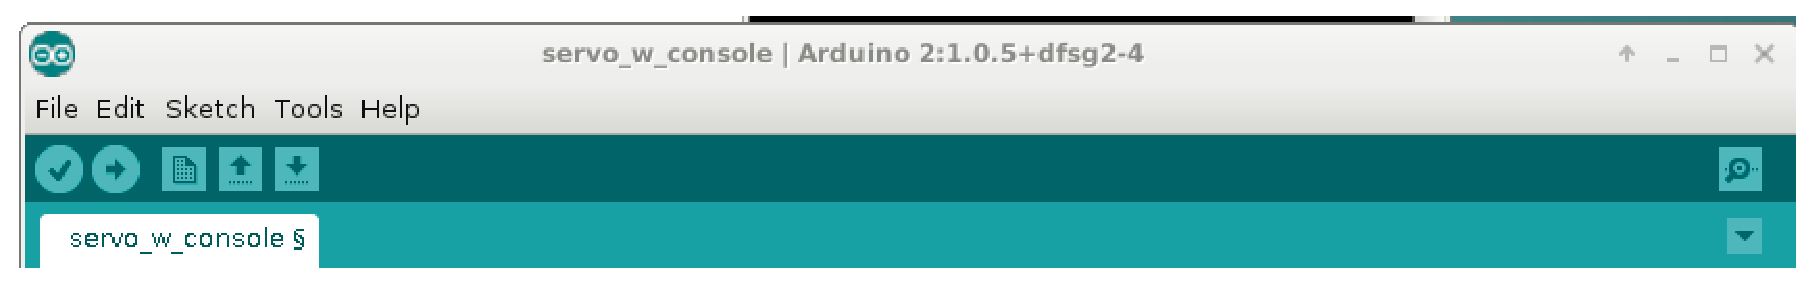
\includegraphics{turnonserialconsole.eps}}
%\rput[bl](0,0){\psgrid(0,0)(30,8)}
	\fontsize{24}{24}\selectfont
	\rput[bl](10,5){\textcolor{blue}{Click here to open the Serial Console}}
	\pnode(14.2,5){A}
	\cnode[linewidth=5pt,linecolor=yellow](29.2,1.6){1}{B}
%	\nccurve[angleA=-90,angleB=90,arrowsize=10pt]{->}{A}{B}
	\ncline[linecolor=red,linewidth=4pt,arrowsize=12pt]{->}{A}{B}
\end{pspicture}
\endTeXtoEPS
\end{document}
